\documentclass[10pt, a4paper,titlepage]{article}

\usepackage{graphicx}
\usepackage{listings}
\usepackage[normalem]{ulem}
\usepackage{caption}
\usepackage[bottom]{footmisc}

\begin{document}
\begin{titlepage}
\title{Design Document \\Version 1.1}
\author{Emanuele Ricciardelli (mat. 875221) \and Giorgio Tavecchia (mat. 874716) \and Francesco Vetr\'o (mat. 877593)}
\begin{figure}
\begin{center}

\includegraphics{/home/francesco/git/Project_SE2_RTV/DD/DD_images/logopolimi.png}
\caption{Politecnico di Milano}
\label{fig:logo}
\end{center}
\end{figure}
\maketitle
\end{titlepage}
\tableofcontents
\pagebreak
\section{Introduction}
\subsection{Purpose}
This document will provide a set of architectural and design details in order to drive software developent of the PowerEnjoy system-to-be. Specifically,  the following will be now identified and described:
\begin{itemize}
\item High level architecture;
\item Main component view;
\item The runtime behaviour of components;
\item Design patterns.
\end{itemize}•
\subsection{Scope}
The system should be able to register new users with their credentials, such as name, surname, address and e-mail, their valid driving license number and some payment information. Once the registration process is completed and all entered data are verified, the system will send a password to the user: this password will be used by the user to access the system and its functionalities. The system provides the following common features: 
\begin{itemize}
\item find an available car;
\item reserve an available car one hour prior the pick up; 
\item unlock the car when the user is detected nearby the car he/she reserved;
\end{itemize}•
In addition there will be incentives for virtuous behaviors of the user that will affect their fares: if an user helps the community by being responsible with the usage of the car, his/her fare will be reduced by a specified percentage; otherwise, by not following the guidelines of the company, the user will be charged more than the standard fare
\subsection{Definitions, acronysm, abbreviations}
\begin{itemize}
\item \underline{\textbf{RASD}}: Requirements Analysis and Specifications Document;
\item \underline{\textbf{Gateway}}: tool to set the communication and the exchange of data between two or more networks with, often, different protocols;
\item \underline{\textbf{Push notification}}: notification sent to a smartphone via application installed on it;
\item \underline{\textbf{Email}}: mail service carried over the web;
\item \underline{\textbf{API}}: Application Programming Interface.  It is a set of subroutine definitions, protocols, and tools for building application software;
\item \underline{\textbf{Google Maps API}}: APIs provided by Google to compute functionalities over the Google Maps environment;
\item \underline{\textbf{MVC}}: Model View Controller pattern;
\item \underline{\textbf{Tier}}: architectural level in which the system is decomposed;
\item \underline{\textbf{Client}}: program or part of a program which allows to exchange data with a server to perform computations;
\item \underline{\textbf{Thin Client}}: client dedicated to only graphical representation, which displays the results of a computational logic contained exclusively in server;
\item \underline{\textbf{Application Server}}: it provides the infrastructure and support functions, development and execution of applications in a distributed environment;
\item \underline{\textbf{Database Server}}: software system able to store and manipulate data contained in a database;
\item \underline{\textbf{Execution Environment}}: it represents a particular execution platform, such as an operating system or a database management system. Execution environments are used to describe the context in which the execution of a model takes place;
\item \underline{\textbf{Controller}}: software system that applies changes to the model and database;
\item \underline{\textbf{UX}}: user experience diagram;
\item \underline{\textbf{BCE}}: Boundary Control Entity diagram;
\item \underline{\textbf{Ticket}}: the term refers to a fine that a driver has received during a ride;
\item \underline{\textbf{Record Maintenance}}: record saved in the Database, used to save information concerning the maintenance processes of a car.
\end{itemize}•
For all terms not specified, please refer to the glossary contained in the previous document (RASD).
\subsection{Reference documents}
\begin{itemize}
\item Specification document: Assignments AA 2016-2017.pdf;
\item RASD previously version 1.0;
\end{itemize}•
\subsection{Document structure}
\begin{itemize}
\item Introduction: this section introduces the design document, providing a brief indication of its utility and about the covered sections;
\item Architecture design:
\subitem - Overview: this sections explains the high level components and their interaction;
\subitem - Component view: more detailed view of the components of the application;
\subitem - Deployment view: this section shows all components that must be deployed to have the application running completely and correctly;
\subitem - Runtime view: it describes how components interact with each other to accomplish specific tasks;
\subitem - Component interfaces: it describes the interfaces between the components;
\subitem - Selected architectural styles and patterns: it provides details related to patterns and architectural styles selected for the development;
\subitem - Other design decisions;
\item Algorithms design: this section provides some algorithms useful to describe some functionalities of the system;
\item User interface design: this section presents a detailed description of user experience explained with diagrams like UX and BCE;
\item Requirements traceability: this section aims to explain how the decision taken in the RASD are linked to design elements.
\end{itemize}•
\newpage
\section{Architectural Design}
\begin{figure}
\includegraphics[scale=0.4, keepaspectratio]{/home/francesco/git/Project_SE2_RTV/DD/DD_images/High_level_components.png}
\caption{High level components}
\label{fig:high_level_components}
\end{figure}
\subsection{Overview}
The PowerEnJoy system will be shaped in a three tier architecture. This architectural style allows a further enhancement: the possibility to move the entire application in a dedicated cloud server with elastic infrastructure in order to get performances needed by the load on the application on demand and the consequent money saving. This choice will also face the coupling problem with respect either to the logic and data level and to the logic and presentation level. Nonetheless a performance evaluation might need to check whether the contract terms are satisfied. Important decision based on this architecture is the thin client characterization: the client can only send to the server a sequences of requests on what operation is intended to perform. This choice can possibly raise the expenses for the company. In the right part of Figure 2 is present the component named as “Payment System”: this component is intended to be a set of functionalities offered to the banks in order to ensure the correctness of all the payment operations. In Figure 3 we show the existence of firewalls in between the layers: this is due to the high security problems that this service arouses. Since our data level will store personal information such as identity, mail address, number of credit cards and even positions of a human being, a possible solution is to use different techniques to ensure that none will ever access private data.
\begin{figure}
\begin{center}
\includegraphics[scale=0.6, keepaspectratio]{/home/francesco/git/Project_SE2_RTV/DD/DD_images/Tier_levels.png}
\end{center}
\caption{Tier levels}
\label{fig:tier_levels}
\end{figure}
\newpage
\subsection{High level components and their interaction}
The high level components architecture in Figure 2 is made of five parts. The main part is the \emph{Global system}: it is a singleton that contains all the business logic. It is splitted into two sections: 
\begin{itemize}
\item the \emph{Car sensors subsystem}, as stated in the RASD, the cars are seen by the system as a set of sensors and actuators that only provide data. This part of the system-to-be is devoted to collect data from cars, convert them in a usable structure for the system and then send them to the business logic part named \emph{Application server};
\item the \emph{Application server} that will receive requests, will manage the information provided by the \emph{Car sensors subsystem} and will be able to communicate with the \emph{Payment system} in order to retrieve payments information.
\end{itemize}•
The customer, via the mobile app or the service’s web page, can initiate a communication with the \emph{Application server} that will complete the task requested and will answer back immediately with a message about the success or failure of the request and, if other information are needed, will send an email or a push notification providing the missing part (e.g. the client reserves a car, the request is successful and the system answers with a push notification/email containing the code to unlock the car).
Then the maintenance service can communicate with the system through their own web application expressly developed in order to this purpose using our API's. Here the maintenance personnel can look at all the stored maintenance requests and change the status of this requests. (e.g. a request of a car left with less than 5\% of the battery might be changed to \textit{performing}, and after the car is put in charge its status will be changed in \textit{complete}).
In the right part of Figure 2 there is the \emph{Payment system}. This system is supposed to interact with banks and the “Application server” in order to perform checks and updates all the information regarding payments. The banks will use this interface to communicate with our system, and the \emph{Payment system} will act as a controller and will request the \emph{Application server} to perform the needed changes to the database in order to maintain the correct status of payments and users. This is due to a previous decision stated in the RASD \textit{(Table 13: Provide a payment)}.
The \emph{Application server} needs to store and perform queries in order to perform all the tasks and so communicates with a database.
\clearpage
\begin{figure}[h]
\begin{center}
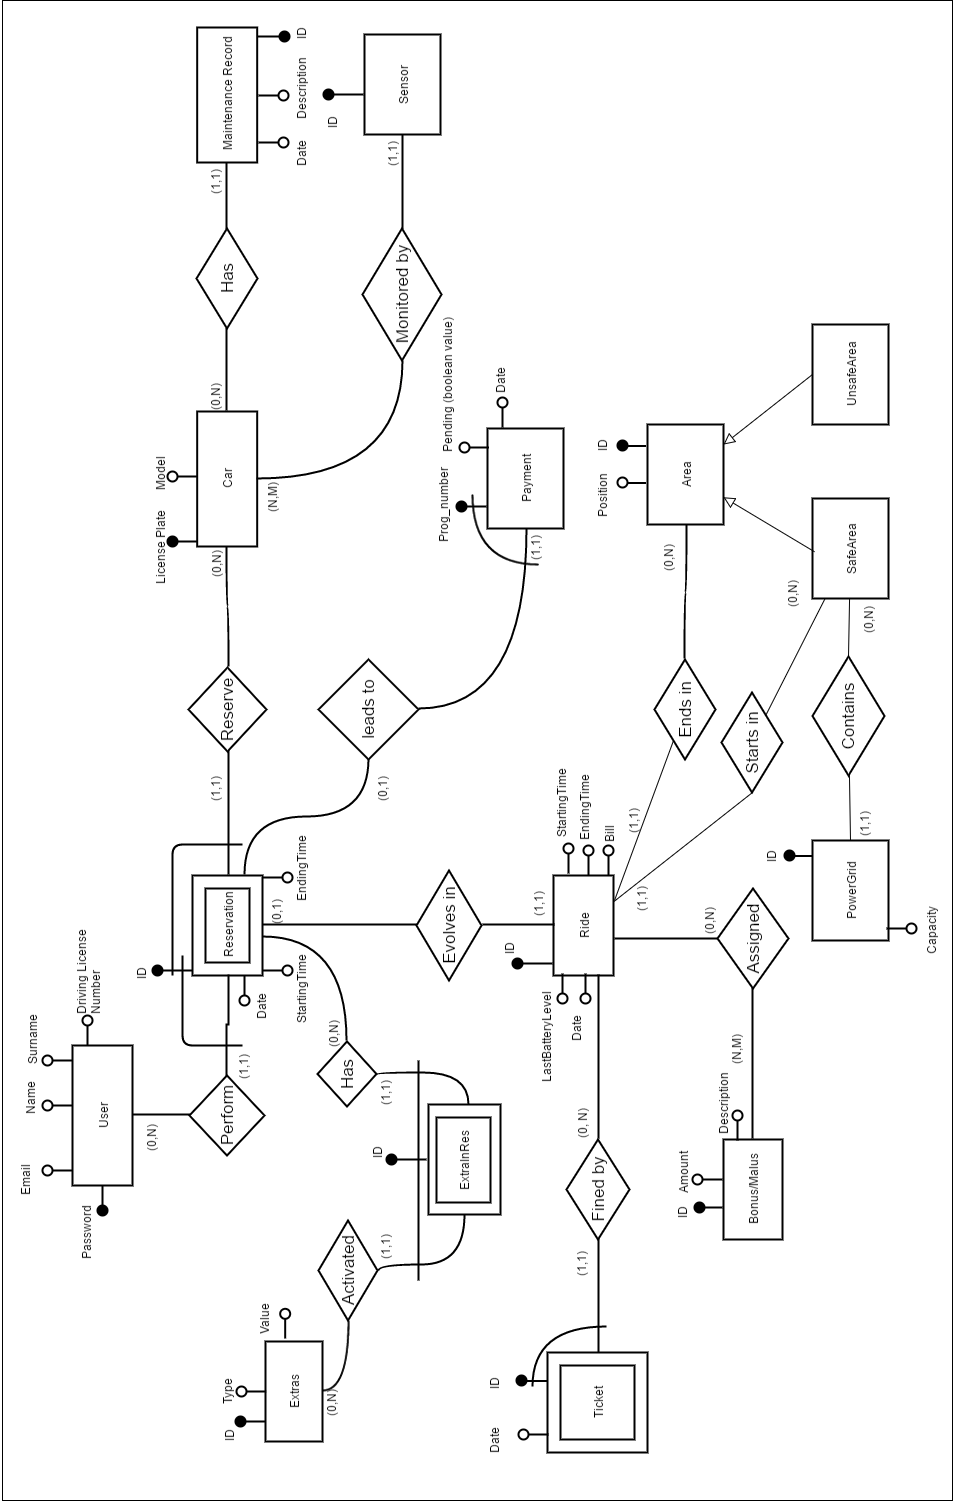
\includegraphics[width=\textwidth,height=0.8\textheight,keepaspectratio]{/home/francesco/git/Project_SE2_RTV/DD/DD_images/ER.png}
\end{center}
\caption{ER diagram}
\caption*{\underline{Observation}: ID in \emph{Reservation} entity, combined with the user and car's informations, will later be converted into QR Code through cryptography algorithms to enable the user to access the car that he has previously reserved. \emph{ExtrainRes} is the set of all the operations that have been performed on a specific reservation that can involve an addition in the payment of the total cost, in our case just the \emph{extension} of the reservation time and the deletion (\emph{delete}) of the reservation itself.}
\label{fig:ER}
\end{figure}
\clearpage
\subsection{Component view}
\begin{figure}[h]
\begin{center}
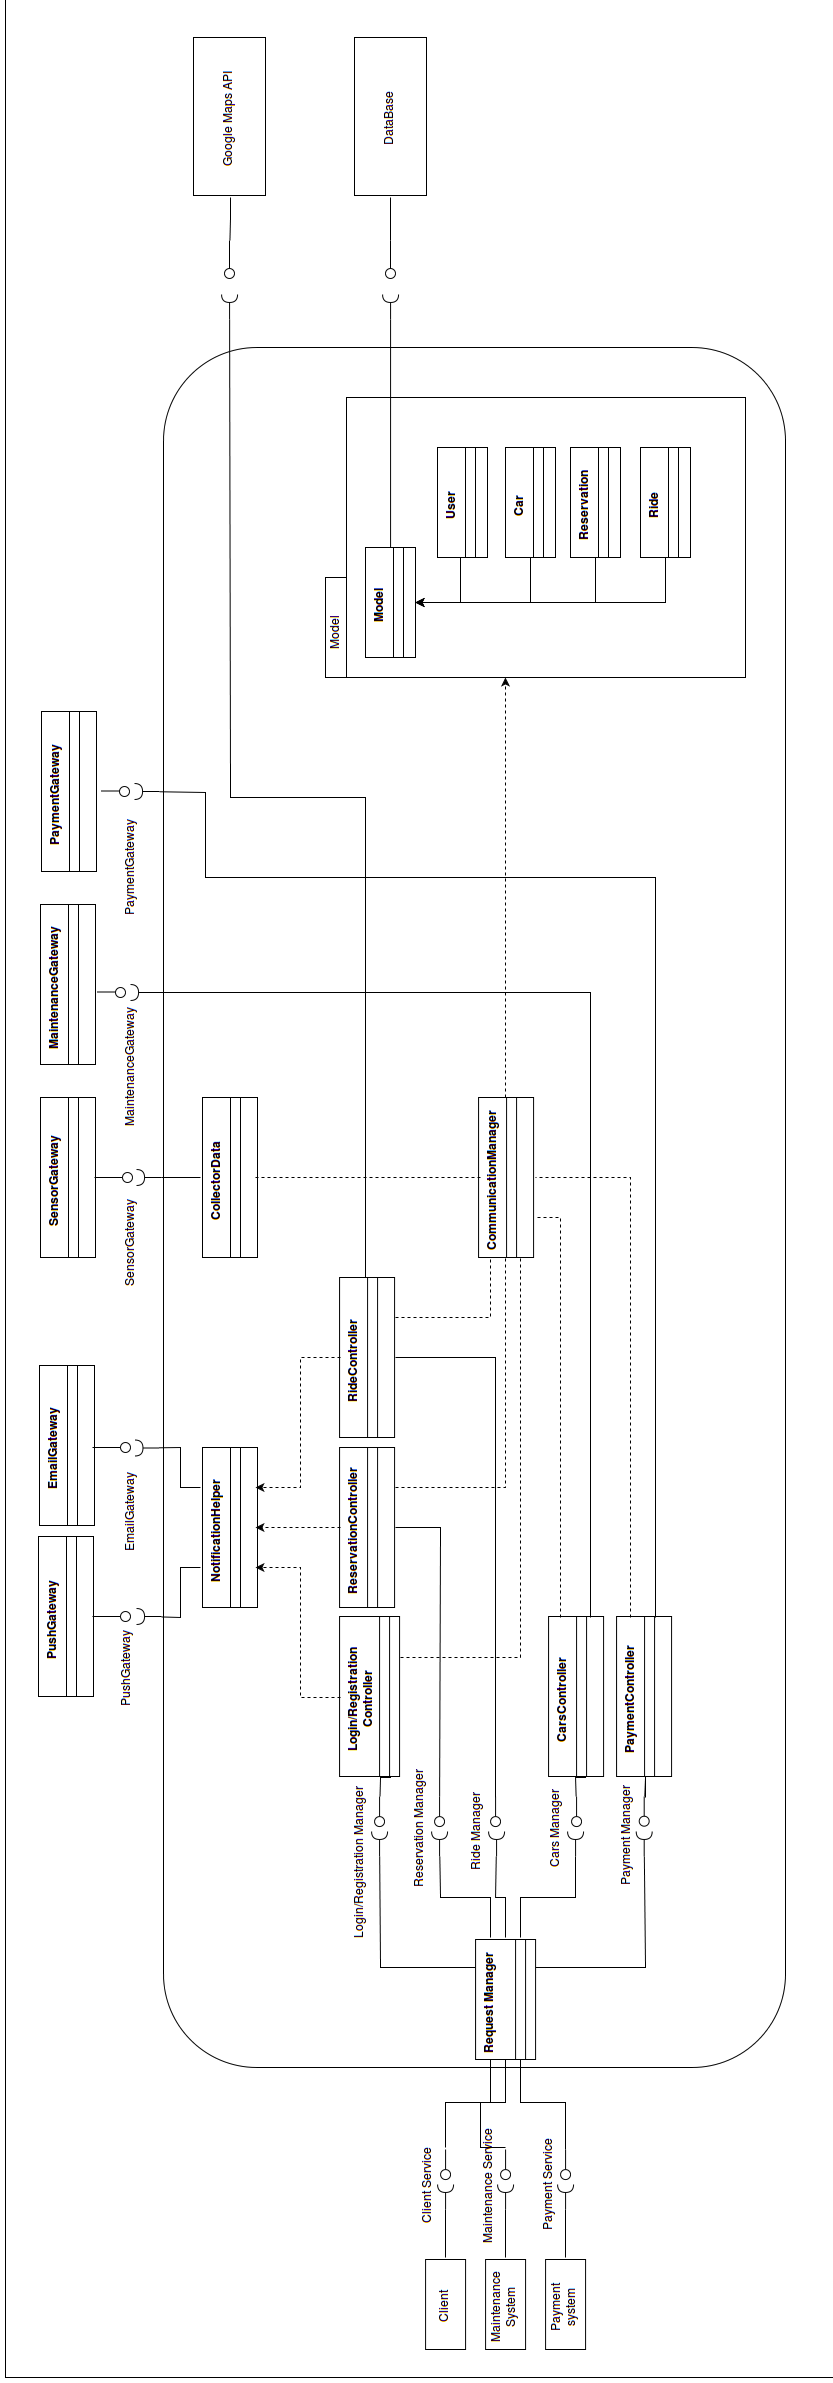
\includegraphics[width=\textwidth,height=0.7\textheight,keepaspectratio]{/home/francesco/git/Project_SE2_RTV/DD/DD_images/Component_view.png}
\caption{Component view}
\label{fig:component_view}
\end{center}•
\end{figure}
\clearpage
The component view consists of the following components:
\begin{itemize}
\item \textbf{Client}: client’s device used to connect to the service
\item \textbf{Maintenance}: maintenance device used to interact with the system in order to provide maintenance features.
\item \textbf{Payment system}: third party device used to provide information about payments, their completion and other relating information.
\item \textbf{Request manager}: manager used to receive request from the outside and to route them to the correct controller. 
\item \textbf{Login/Registration controller}: \sout{manage login and registration aspects.} Controller used for the management of the operations related to login and the system registration.
\item \textbf{Reservation controller}: \sout{manage reservation aspects.} Controller used for the reservation management , such as creating, by searching available cars or retrieving the unlock code, deleting, and extension.
\item \textbf{Ride controller}: \sout{manage ride aspects.} Controller used for the management of rides. It contains functions for the initiation and termination of rides. In addition, it implements methods for enabling the \emph{Money-saving option}.
\item \textbf{Cars controller}: manage all informations related to cars, sensors, actuators and their interaction with the users.
\item \textbf{Collector data}: manage the data collection from different sensors and actuators.
\item \textbf{Payment controller}: manage payment aspects like register debts or mark their completion.
\item \textbf{Communication manager}: component used to manage information exchange between different controllers and between them and the \sout{model.} data access manager.
\item \textbf{Notification helper}: manage notification aspects, routing them to the correct gateway
\item \textbf{Push gateway}: manage the sending of push notification to mobile app.
\item \textbf{Email gateway}: manage the sending of Email messages.
\item \textbf{\sout{Sensor} Car gateway}: handle the sending and receiving of data collected by the various sensors present on cars.
\item \textbf{Maintenance gateway}: manage the sending of notification to the maintenance company
\item \textbf{Payment gateway}: manage the sending of payment information to the third party payment service
\item \textbf{\sout{Model} Data Access Manager}: \sout{model of the world, used by the controllers.} Component used to manage and access the database. It is used to mantain the actual model the system is working on.
\item \textbf{Database}: database used to store persistent data.
\item \textbf{Google Maps API}: API service used by the ride controller to provide navigation information.
\end{itemize}•
The interaction between the system and users is provided by a series of interfaces, one for each type of actor. All requests are handled by the single component \emph{Request Manager} that will provide for their proper forwarding within the system. We have designed a system consisting of several controllers, each dedicated to a specific type of functionality. This allows us to maintain a high level of cohesion of the different components, allowing, in case of future expansions of the service, to update the individual components smoothly and with great flexibility. The division of functions in various components will also allow us to efficiently test the service provided. In order to maintain a high degree of flexibility, we decided to introduce a component \emph{Communication manager} dedicated to the sorting of the information exchanged between the controllers themselves and the \sout{model} Data access manager, thus avoiding the definition of direct links between controllers that might obstruct and make more complex a future possible expansion of the service. A little remark concerns the system’s design, in detail concerning of the Collector Data component: despite the most part of the functionalities is strictly linked to the Cars Controller component, we have decided to instantiate a connection between Collector Data and Communication Manager. This allows the Reservation Controller, in the new reservation’s creation step, to communicate directly the unlocking code to the car without passing through other intermediate components. This choice eases the workload of the Cars Controller, that is the central hub of the whole operations concerning the reservation and ride subsystem. 
In analogous way we introduced a component \emph{Notification helper} dedicated to the proper addressing of the notifications to users, thus separating the functionality of sending of notifications from the logic of the underlying service.
As shown in the diagram, the only access to the \sout{model and to the database it} database of the system is via the \emph{Communication Manager} that will \sout{carry out read and write functionality.} forward all the possible queries to the data access manager.
All the operations performed by the Payment Controller are based on an identifier generated by our system and mapped with the User ID (i.e. the password). The ID generated is then communicated to the Payment Society in order to the decouple the user’s informations and to avoid sensitive data exposition.
\newpage
\subsection{Deployment view}
\begin{figure}[h]
\begin{center}
\includegraphics[width=\textwidth, height=0.7\textheight, keepaspectratio]{/home/francesco/git/Project_SE2_RTV/DD/DD_images/Deployment_view.png}
\caption{Deployment view}
\label{fig:deployment_view}
\end{center}•
\end{figure}
\newpage
\subsection{Runtime view}
\subsubsection{Login}
\begin{figure}[h]
\begin{center}
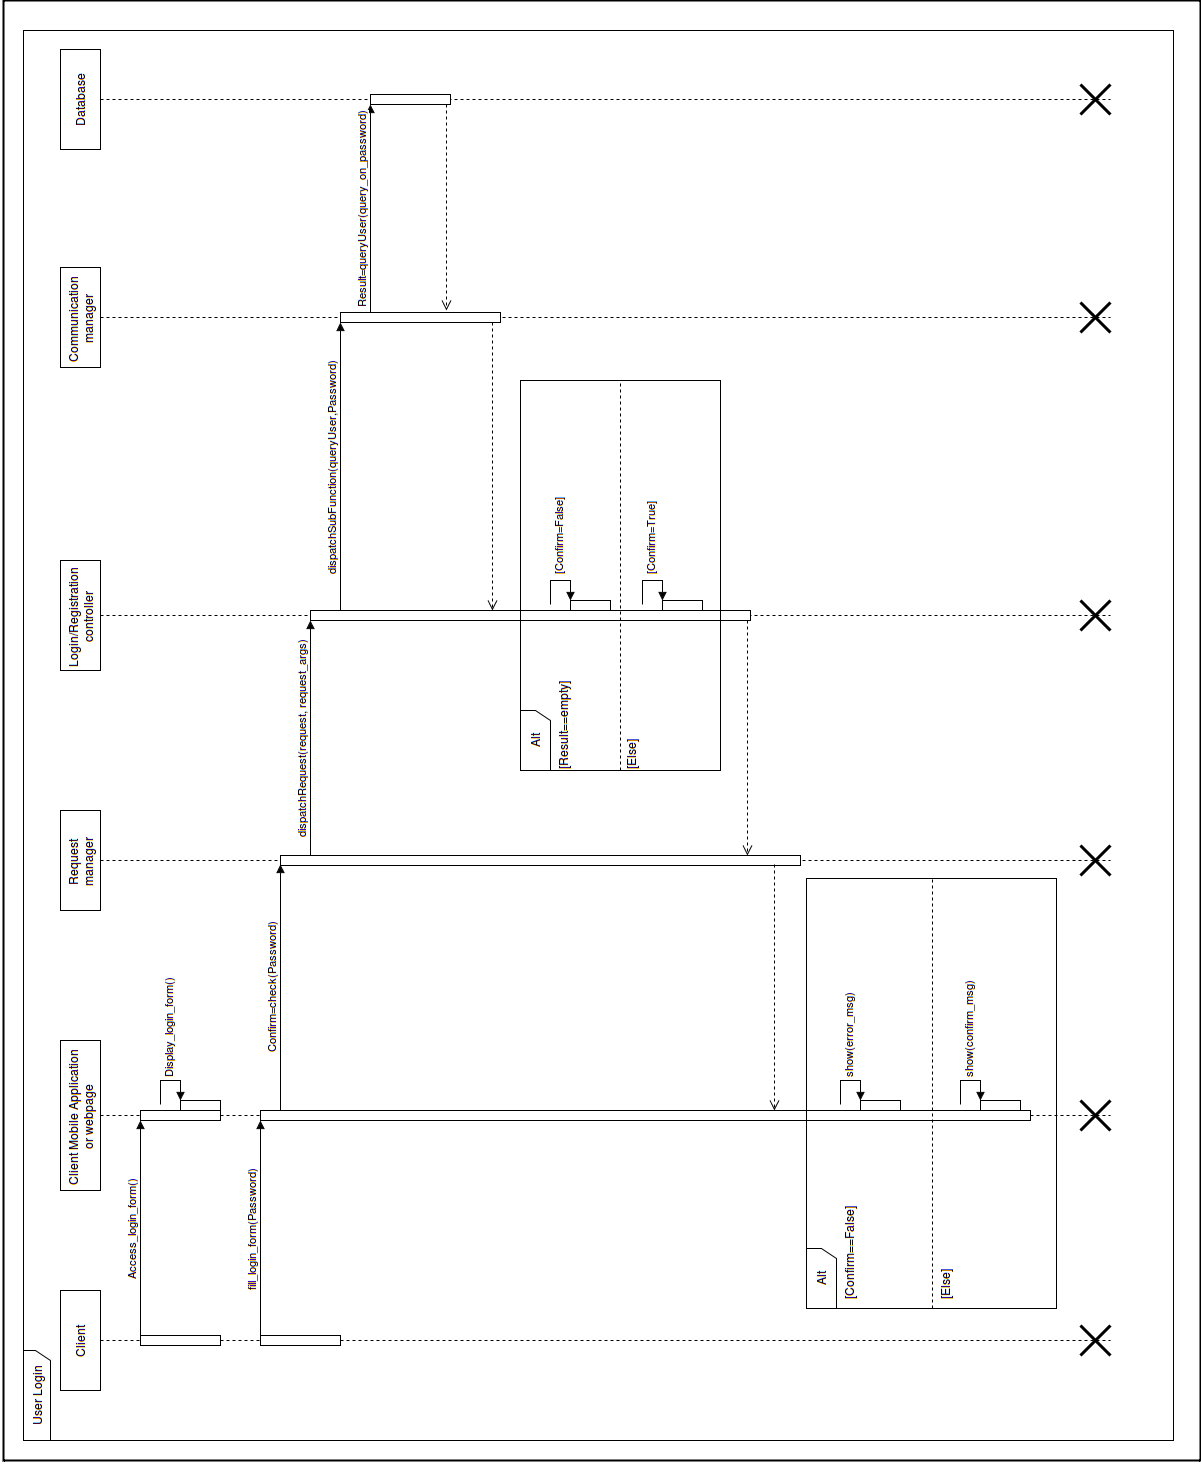
\includegraphics[width=\textwidth, height=0.7\textheight, keepaspectratio]{/home/francesco/git/Project_SE2_RTV/DD/DD_images/sequence_diagram_login.png}
\caption{Sequence diagram - login}
\label{fig:sequence_diagram_login}
\end{center}•
\end{figure}
In this sequence diagram it is represented the interaction among the components of the system in order to verify the correctness of the password entered by a user.
After completing the login form, the request is forwarded to the \emph{Request manager} that, once identified, will forward it to the correct controller (in this case the\emph{Login / Registration controller}).
It, to deal with the request, will perform a query on the database of the system in order to verify the presence or absence of a user with corresponding password to the one supplied.
The new request is then forwarded to the \emph{Communication manager} that ultimately will apply it to the DB.
The query result will be interpreted by the \emph{Login / Registration controller} that will send the confirmation, or not, of the login to the interface which started it.
In this sequence diagram it is not represented the collection of all the information needed to display the user's homepage because it will be made only after effective login confirmation.
\subsubsection{Report car issue}
\begin{figure}[h]
\begin{center}
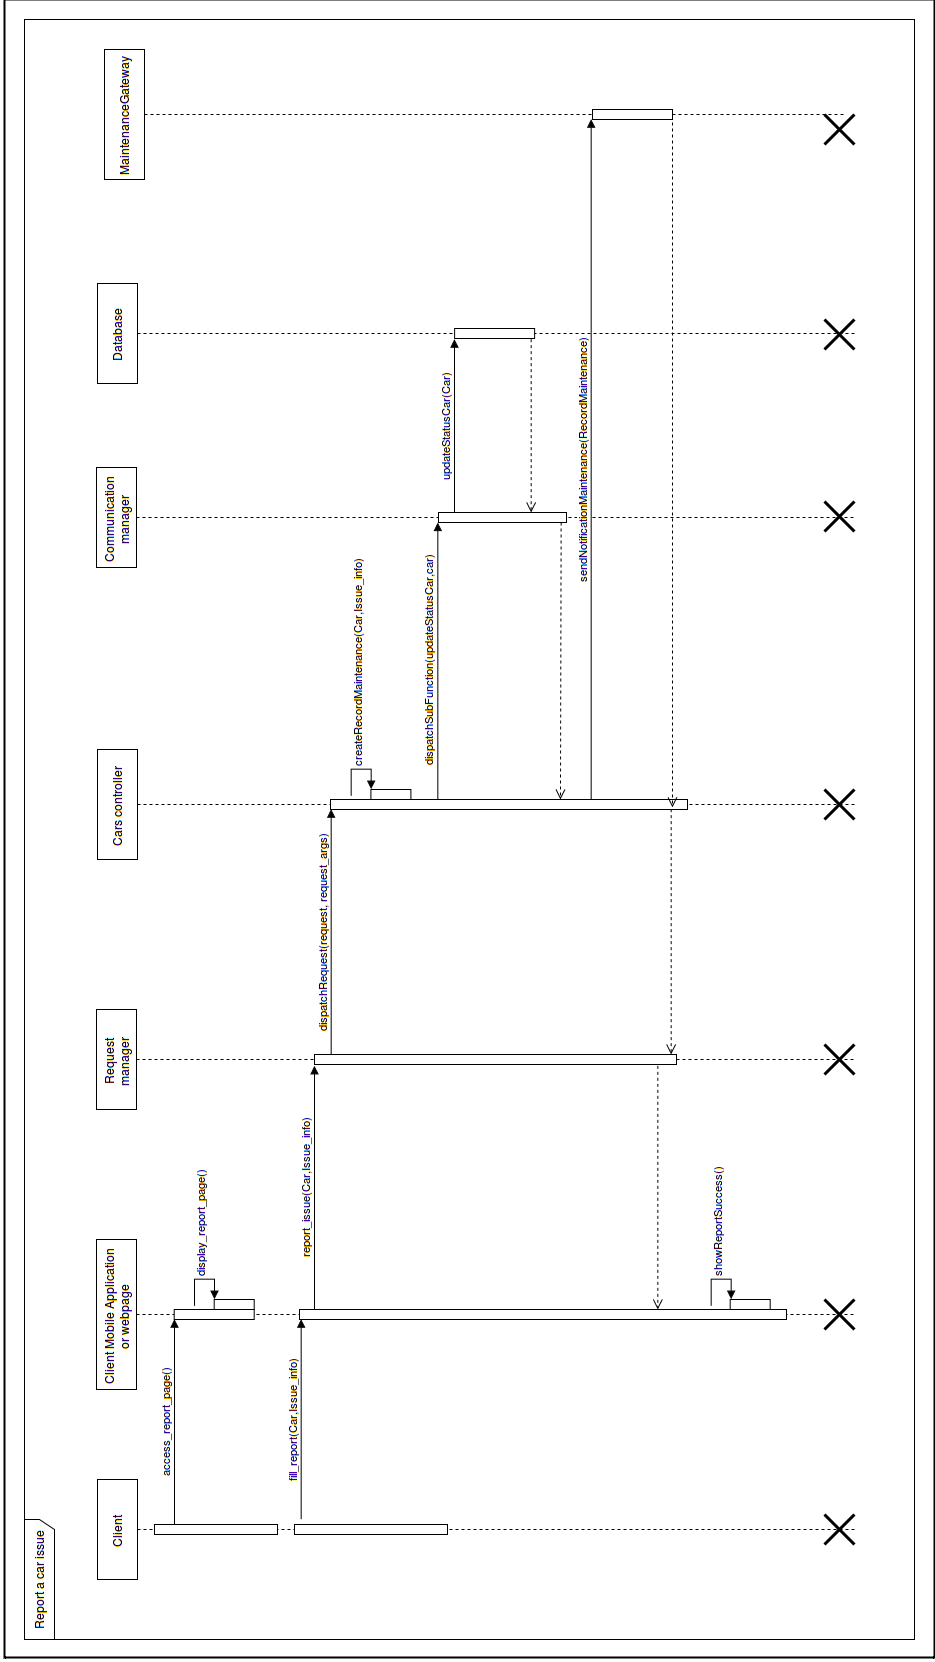
\includegraphics[width=\textwidth, height=0.7\textheight, keepaspectratio]{/home/francesco/git/Project_SE2_RTV/DD/DD_images/sequence_diagram_report.png}
\caption{Sequence diagram - report car issue}
\label{fig:sequence_diagram_report}
\end{center}•
\end{figure}
In this sequence diagram it is shown the flow of information and instructions exchanged between the components for reporting car issue.
The report starts from a user, that, with his own application fills out a form with all the details regarding the car and the problem.
The request is now forwarded to the \emph{Car controller} that will seek to create a record for maintenance and will save it to the database, associating it to the corresponding car.
Once this is done, the same \emph{Car controller} will perform a notification to the maintenance company that later will have access to the report and provide for the resolution of the problem.
\subsubsection{Money saving option}
\begin{figure}[h]
\begin{center}
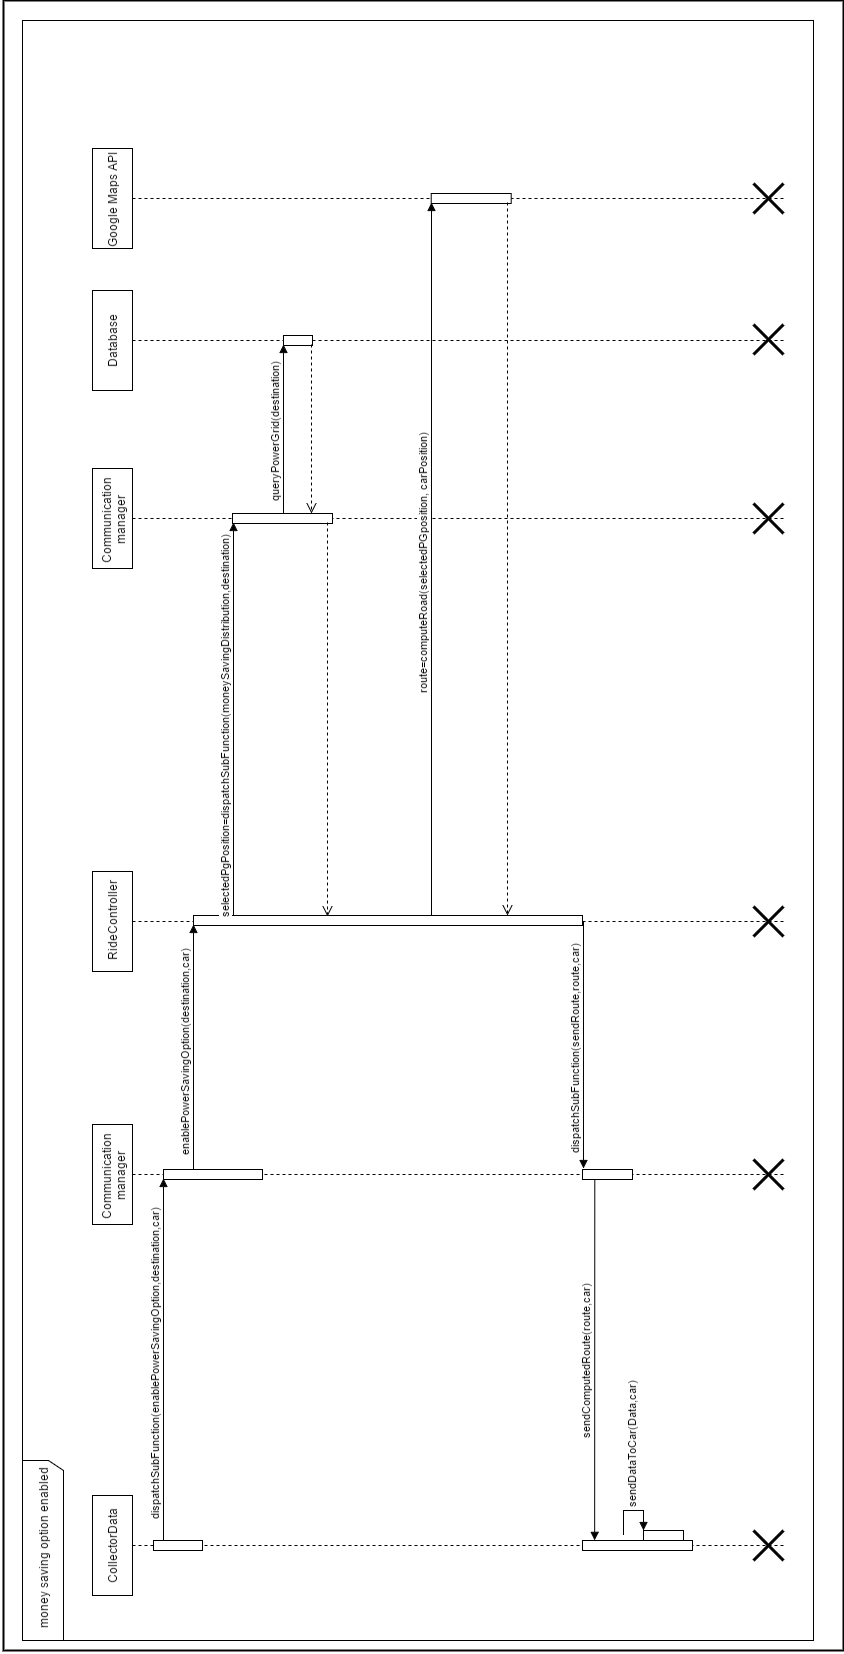
\includegraphics[width=\textwidth, height=0.7\textheight, keepaspectratio]{/home/francesco/git/Project_SE2_RTV/DD/DD_images/sequence_diagram_saving.png}
\caption{Sequence diagram - money saving option}
\caption*{\underline{Observation}: \emph{Communication manager} is here duplicated only for meanings of readability, in the system-to-be is only a single instance.}
\label{fig:sequence_diagram_saving}
\end{center}•
\end{figure}
This sequence diagram shows the flow of instructions that allow the activation of the “money-saving” option during a ride.
The user must provide his final destination in order to compute the shortest route to the nearest powegrid station to his destination.
Once the driver has selected his destination, the system in the vehicle will interface to the PowerEnJoy server to provide the selected service: the request is received by the “CollectorData” which in turn will communicate to the “RideController”; the features of this controller are not limited only to the definition of rides and their stages, but will contain all the logic required for the above described functionality.
The “Ride Controller” will perform the proper algorithm developed to find the right PowerGrid in order to reach the purpose of this functionality. Once that is done, the algorithm will have figured out the position information of the proper PowerGrid and then the controller will interface with the APIs provided by Google Maps to compute the road.
Finally, it will send the result of this computation to the driver who asked it.
\clearpage
\subsection{Component interfaces}
\sout{In this section are explained two kind of interfaces: first the interfaces that which the system provides to the applications that connect to it; , second the interfaces which each component provides in order to make easier the communications through different component. For each of them it is described the methods that are made available and the parameters necessary for their proper execution.} In this section are included all the interfaces that each component of the system expose in order to make easier the communications through different component. For each of them it is described the methods that are made available and the parameters necessary for their proper execution. 
\begin{figure}[h]
\begin{center}
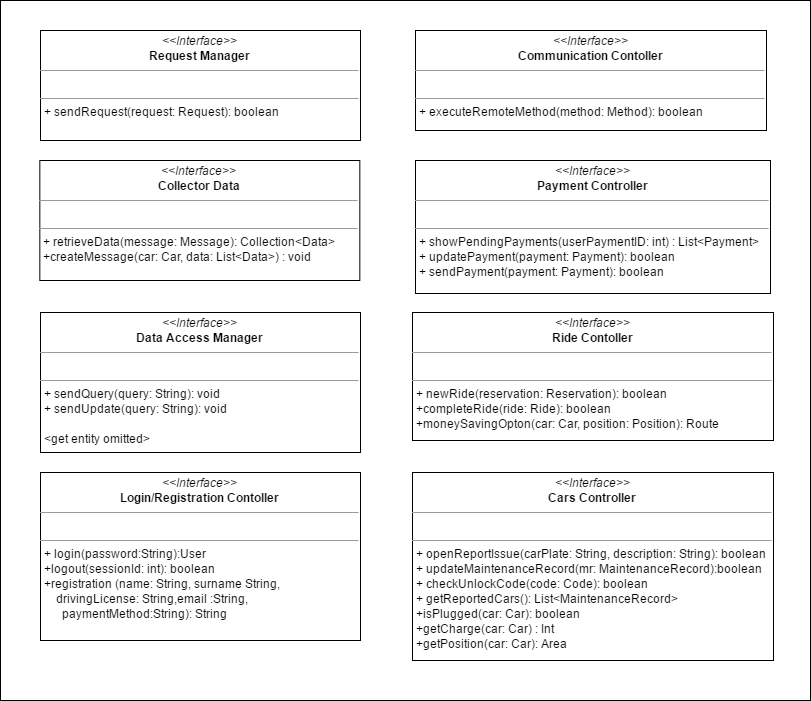
\includegraphics[width=\textwidth, height=0.5\textheight, keepaspectratio]{/home/francesco/git/Project_SE2_RTV/DD/DD_images/INTERFACCE1.png}
\caption{Component interfaces - 1}
\label{fig:scomponent_interfaces}
\end{center}•
\end{figure}
\begin{figure}[h]
\begin{center}
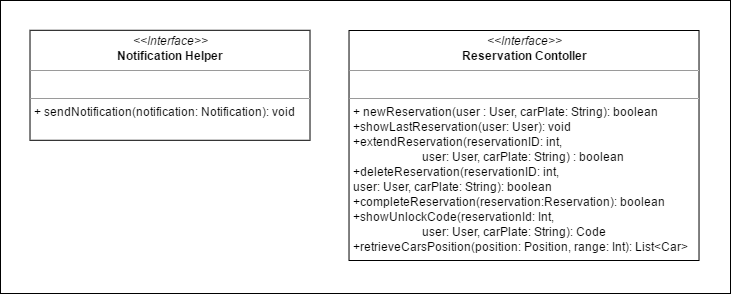
\includegraphics[width=\textwidth, height=0.5\textheight, keepaspectratio]{/home/francesco/git/Project_SE2_RTV/DD/DD_images/INTERFACCE2.png}
\caption{Component interfaces - 2}
\label{fig:scomponent_interfaces}
\end{center}•
\end{figure}
\begin{figure}[h]
\begin{center}
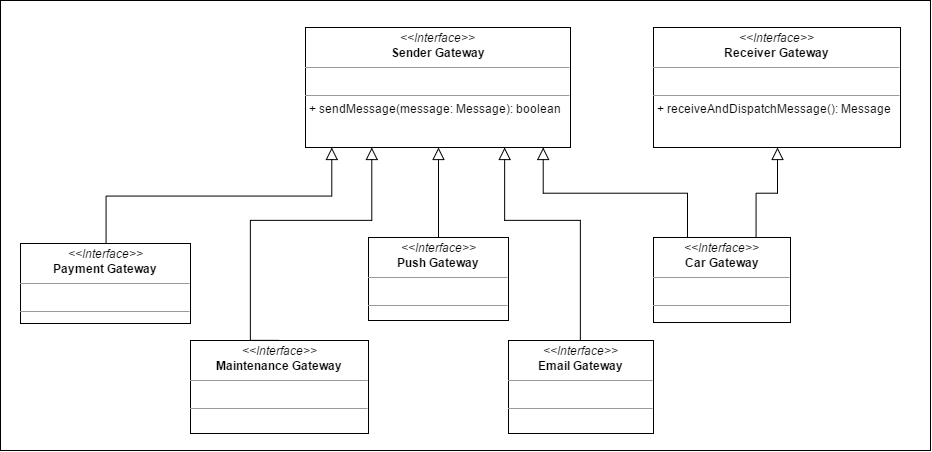
\includegraphics[width=\textwidth, height=0.5\textheight, keepaspectratio]{/home/francesco/git/Project_SE2_RTV/DD/DD_images/INTERFACCE3.png}
\caption{Component interfaces - 3}
\label{fig:scomponent_interfaces}
\end{center}•
\end{figure}
\clearpage
\subsection{Selected architectural styles and patterns}
Reflecting on the architectural design of the system-to-be, we identified some styles and patterns that best reflect our idea of design, as well as provide us with a solid structure on which to base our development.
\subsubsection*{Client-Server}
Since the first description of the system-to-be we identified in the model a distinction between the logic of the system and the users themselves; this type of functionality distinction is reflected in the architecture of client-server.
In particular, we decided to develop an architecture based on 3-Tier where the client is of type “thin”.
This allowed us to keep the client side as light as possible, so as to concentrate the computational power of the devices on only GUI aspects. 
On the other hand, the large computational load required by the servers will be guaranteed, both from a reliability and efficiency point of view, through the use of cloud computing, which will allow us to have an easily scalable service.
A client server architecture of this type, in addition to the advantages mentioned above, allows us to guarantee a high level of security, because the clients do not directly access the data contained in the database as well as have no dependence on each other.
Finally, since the clients use interfaces provided by the server, and does not compute any functional activity, future service enhancement will be completely transparent to all clients themselves.
\subsubsection*{Adapter}
As visible in the \emph{Component View} (\S 2.3), we designed our system dividing the functions that must be provided in multiple controllers,each covering a single aspect of the system.
This, as previously described, allows us to maintain a high degree of cohesion between the various components, as well as allowing us to manage them in a more elastic way.
However, the breakdown of the more system controllers introduces a problem concerning the exchange of information between them. The system will not present direct links between these but, through the “Communication Manager” will implement the Adapter pattern. This will permit to separate the development of a component from the surrounding ones, to which ,using interfaces, will be fully transparent.
\subsubsection*{MVC}
The Model-View-Controller pattern will cover an important role in our system. As described in the component view, we decide to separate the internal representations of data from the ways that information is provided to the users. 
The view is composed by all kind of clients that can connect and operate on the system-to-be.
The controller part is our application server and it contains all the logic of the system.
The model cover the rule of managing the data of the service itself.
With the use of this pattern we do not permit any direct access to data from clients, without going through the controller section.
\subsection{Other design decisions}
Since that our service must ensure a high degree of efficiency, both in terms of response times and of the number of users connected simultaneously, we suggest the development of the web server on NginX.
This type of web server is in fact able to ensure indexes of performance as mentioned above, basing its computation on an asynchronous approach to events.
The server will be based on non-blocking operations, thus able to not slow down the overall operation in case of high level of parallelism, as it would happen in Apache web server.
\section{Algorithms design}
In this section we want to provide a short description of some useful code that will be implemented in the future system.
\addcontentsline{toc}{subsection}{Discounts' assignation}
\subsection*{Discounts' assignation}
This algorithm will manage to properly assign discount at the end of a ride:
\begin{lstlisting}[language=Java][width=\textwidth]
public List<Discount> computeDiscounts(Ride ride){
    List<Discount> discounts=new ArrayList<Discount>();
    Car car=ride.getCar();
    
    if(car.isInCharge())
        discounts.add(new PowerGridDiscount());
    else{
        if(car.getPosition().distanceFromNearestPG()>3){//3km
            discounts.add(new MalusDistance3());
        }
        else{
            if(car.getCharge()<=20)   //20%
                discounts.add(new MalusBattery20());
        }
        if(car.getCharge()>=50)   //50%
            discounts.add(new Battery50Discount());
    }
    if(ride.numPassengers()>2)
        discounts.add(new PassengersDiscount());
        
    return discounts;
}
\end{lstlisting}
\bigskip
\bigskip
\addcontentsline{toc}{subsection}{Ride's end}
\subsection*{Ride's end}
This algorithm will enclose all the functions required to terminate a ride. We consider the execution starting point as the moment at which it takes place the closure signal provided by the concerned machine.
\begin{lstlisting}[language=Java][width=\textwidth]
public void endRide(Reservation res){
    Ride ride=res.getRide();
        if(ride==null) return;


    if(!ride.getCar().getPosition().isSafeArea())
        MaintenanceManager.report(ride.getCar());
    


    List<Discount> discounts=new ArrayList<Discount>();
    
    //Set informations
    ride.setFinalPosition(ride.getCar().getPosition());
    ride.setEndingTime(System.currentTime());
    
    //Computation price
    float price=res.calculatePrice();
    
    discounts=DiscountManager.computeDiscounts(ride);
    for(Discount d: discounts)
        price += d.getValue()*price;        
    
    res.register(price);//Will notify the payment system
    res.close();//Storage on DB
}


public float calculatePrice(){
    float totalPrice=0;
    Ride ride=this.getRide()
    totalPrice+=ride.getBill();//Bill related to the only travel time
    List<Extras> extras=ExtraInRes.getAllExtras(this.getId());
    for(Extras e:extras){
        totalPrice+=e.getValue();   
}
    return totalPrice;
}
\end{lstlisting}
\bigskip
\emph{ExtrainRes} is the set of all the operations that have been performed on a specific reservation that can involve an addition in the payment of the total cost, in our case just the \emph{extension} of the reservation time and the deletion (\emph{delete}) of the reservation itself. 
\addcontentsline{toc}{subsection}{Reservation's extension}
\subsection*{Reservation's extension}
This code will be executed when a user want to extend his reservation.
\begin{lstlisting}[language=Java][width=\textwidth]
public void extendReservation(Reservation res){
    res.setEndingTime(
	new Time(res.getEndingTime().getHour+1,
		res.getEndingTime().getMinute(),
		res.getEndingTime().getSecond());

    ExtraInRes.createNewExtra("extension", res.getId());
}
\end{lstlisting}
\bigskip
\bigskip
This algorithm, as previously mentioned in the RASD, will prevent a user carries out a number of reservations, without extending them, causing financial damage to the company.
\begin{lstlisting}[language=Java][width=\textwidth]
public Reservation newReservation(User user,Car car){
    if(lastCarReserved(user).equals(car) && 
	timeLastExpiredReservation(user)<30)
        return null;
    else
        return new Reservation(user,car);
}
\end{lstlisting}
\addcontentsline{toc}{subsection}{Money saving option}
\subsection*{Money saving option - Car's distribution}
This algorithm will implement the uniform distribution of cars when enabling the money-saving option.
\begin{lstlisting}[language=Java][width=\textwidth]
public Position moneySavingDistribution(Position destination){
    
    List<PowerGrid> powerGrids=DBManager.getAllPowerGrid();
    List<PowerGrid> selected=new ArrayList<>();
    for(PowerGrid pg: powerGrids){
        if(pg.isReachable(destination))
            selected.add(pg);
    }

    HashMap<SafeArea,Integer> map=new HashMap<>();
    for(PowerGrid pg: selected){
	SafeArea s=DBManager.getAreaByID(pg.getAreaID());
		if(map.get(s)==null){
    			map.put(s,pg.getCapacity());
		}else{
    			int val=map.get(s);
			val+=pg.getCapacity();
			map.put(s,val);
		}
    }

    SafeArea safeWithMin=s;
    int min=DBManager.getNumberOfCars(s);
    for(SafeArea s2: map.keySet()){
	int cars=DBManager.getNumberOfCars(s2);
    	if(cars<map.get(s2)){
        		if(cars<min){
			safeWithMin=s2;
        			min=map.get(s2);
		}
    	}
    }
    return safeWithMin.getPosition();
}
\end{lstlisting}
\clearpage
\section{User interface design}
\subsection{Mockups}
\begin{figure}[h]
\begin{center}
\includegraphics[width=\textwidth, height=0.5\textheight, keepaspectratio]{/home/francesco/git/Project_SE2_RTV/DD/DD_images/mockup_homeweb.png}
\caption{Mockup - Home page web application}
\label{fig:mockup_homeweb}
\end{center}•
\end{figure}
\begin{figure}[h]
\begin{center}
\includegraphics[width=\textwidth, height=0.5\textheight, keepaspectratio]{/home/francesco/git/Project_SE2_RTV/DD/DD_images/mockup_reservationweb.png}
\caption{Mockup - Reservation page web application}
\label{fig:mockup_reservationweb}
\end{center}•
\end{figure}
\begin{figure}[h]
\begin{center}
\includegraphics[width=\textwidth, height=0.5\textheight, keepaspectratio]{/home/francesco/git/Project_SE2_RTV/DD/DD_images/mockup_reservationwebok.png}
\caption{Mockup - Reservation successful page web application}
\label{fig:mockup_reservationwebok}
\end{center}•
\end{figure}
\begin{figure}[h]
\begin{center}
\includegraphics[width=\textwidth, height=0.5\textheight, keepaspectratio]{/home/francesco/git/Project_SE2_RTV/DD/DD_images/mockup_manageweb.png}
\caption{Mockup - Manage reservation page web application}
\label{fig:mockup_manageweb}
\end{center}•
\end{figure}
\clearpage
\begin{figure}[h]
\begin{center}
\includegraphics[width=\textwidth, height=1.5\textheight, keepaspectratio]{/home/francesco/git/Project_SE2_RTV/DD/DD_images/mockup_mobile.png}
\caption{Mockup - Mobile app}
\label{fig:mockup_mobile}
\end{center}•
\end{figure}
\begin{figure}[h]
\begin{center}
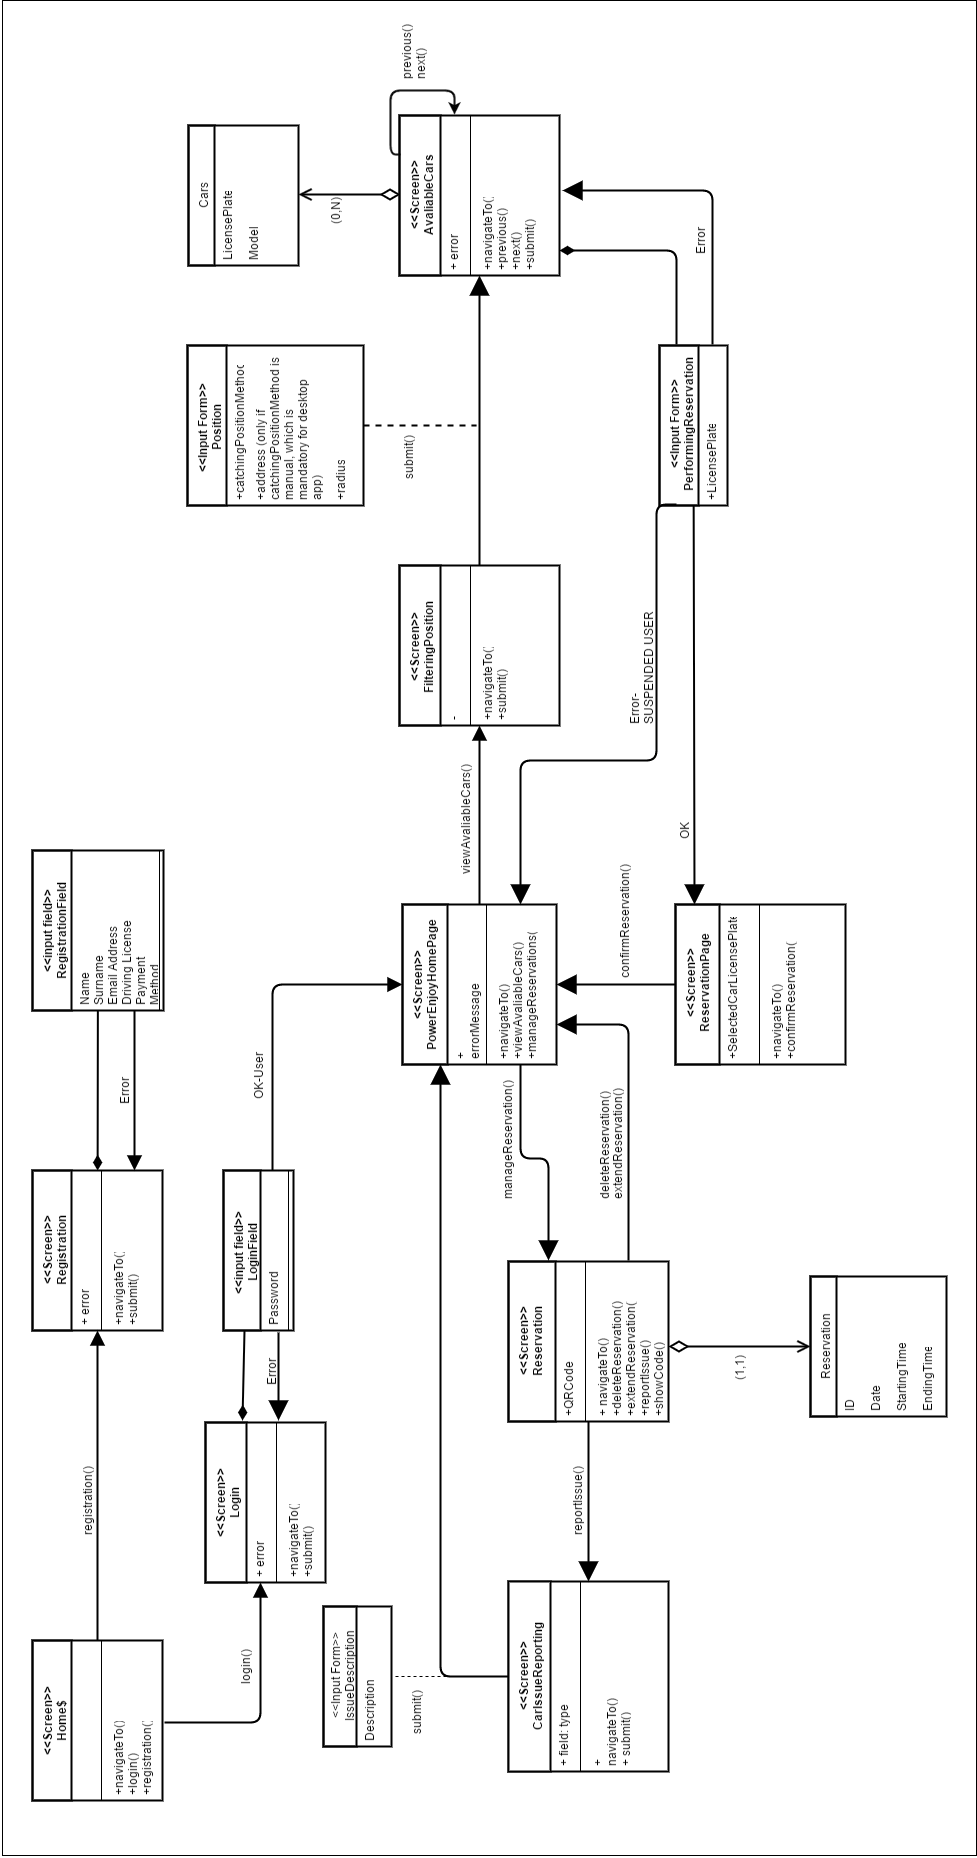
\includegraphics[width=\textwidth, height=\textheight, keepaspectratio]{/home/francesco/git/Project_SE2_RTV/DD/DD_images/UX.png}
\caption{UX}
\label{fig:UX}
\end{center}•
\end{figure}
\clearpage
\subsection{APIs}
\subsubsection{Maintenance system}
In order to keep all the cars working and having a more accessible service, as number of cars available for a user, we have decided to rely on the operations of an external company that will work on the maintenance of the cars. We decided to furnish the company with our API for car maintenance such that all the information about a \emph{malfunctioning} car are handled by our partner. In this case, the term \emph{malfunctioning} means all possible problems that our electric cars can face: for instance the battery charge is below the 5\% or other problems that the \emph{car sensors subsystem} stated in \emph{high level components diagram} in Figure ~\ref{fig:tier_levels} at page ~\pageref{fig:tier_levels} or even a user-reported problem. Our system-to-be will store the information regarding all the \emph{malfunctions} and will interact with the \emph{maintenance system} via our API. The maintenance company will be able to read the problems related to every car and will modify the status of the problem: e.g. a car has a battery charge below 5\%, the maintenance personnel will mark as \emph{Work In Progress (WIP)} the record of the service, the personnel will perform all operations needed in order to put the car in charge and then will mark the record as \emph{completed} so that the car can be available again. The operations performed by the maintenance company are of no interest for our system: what matter is the fact that the car is out of service for a variable period of time and then back available again.
\subsubsection{Payment system}
In order to keep track of all performed payments and to ensure a \emph{fair} use of the PowerEnJoy service, our system-to-be will be interfaced with different payment systems (right part of \emph{high level components diagram} in Figure ~\ref{fig:tier_levels} at page ~\pageref{fig:tier_levels}). The \emph{fair} term, in this context, is based on the fact that an user can possibly have pending payments: in this case the system will not allow the insolvent user to request for other reservation. We will furnish all recognized payment systems with our API for money transfers that will send a request to the user-specified payment system of a bill that must be paid. The payment system will answer and, if the answer is positive and the transaction has been successful, the client is able to continue using our car sharing service. Otherwise, in a negative answer situation from the payment system, our system will temporary suspend the user from the service, until a new and affirmative notification from the payment system will be received. 
\section{Requirements traceability}
This last section is devoted to the representation of how the goals and requirements identified and expressed in previous document (RASD) now find their concretization in the design choices made.
Provided below is a list of goals previously identified and, for each of them, there are expressed the components and architectural aspects which allow their realization
\begin{itemize}
\item[{[G1]}] Guest must be able to register himself in the system.
\subitem - Request Manager 
\subitem - Login/Registration Controller
\subitem - Notification Helper
\subitem - Request Manager 
\subitem - Login/Registration Controller
\subitem - Notification Helper
\item[{[G2]}] User must be able to log in and use the system, if registered.
\subitem - Request Manager
\subitem - Login/Registration Controller
\subitem - Reservation Controller
\subitem - Notification Helper
\subitem - Communication Manager
\item[{[G3]}] User must be able to insert a specified address or his current location to find available cars within a certain distance selected by the user himself.
\subitem - Request Manager
\subitem - Reservation Controller
\subitem - Communication Manager
\subitem - Cars Controller
\item[{[G4]}] User must be able to reserve a car for up one hour in advance.
\subitem - Reservation Controller
\subitem - Notification Helper
\item[{[G5]}] User must pay a fee of 1 euro if the reserved car is not picked up within an hour from the reservation.
\subitem - Reservation Controller
\subitem - Communication Manager
\subitem - Payment Controller
\subitem - Cars Controller
\item[{[G6]}] User must be able to extend his reservation with the payment of a further charge.
\subitem - Request Manager
\subitem - Reservation Controller
\subitem - Communication Manager
\subitem - Payment Controller
\subitem - Cars Controller
\item[{[G7]}] User must be able to notify to the system that he is nearby a reserved car in order to pick it up.
\subitem - Reservation Controller
\subitem - Cars Controller
\subitem - Communication Manager
\subitem - Collector Data
\item[{[G8]}] User must be able to visualize the current charge of his fare.
\subitem - Ride Controller
\subitem - Communication Manager
\subitem - Collector Data
\item[{[G8]}] As soon as the engine ignites, the charge is calculated based on the duration of the service.
\subitem - Reservation Controller
\subitem - Ride Controller
\subitem - Communication Manager
\subitem - Collector Data
\item[{[G9]}] User must be notified if his reserved car becomes out of service and it is no longer available.
\subitem - Cars Controller
\subitem - Communication Manager
\subitem - Request Manager
\subitem - Maintenance Gateway
\subitem - Notification Helper
\item[{[G10]}] User must be able to notify to the company if the reserved car is damaged or not properly working, during their ride or before to pick up the car.
\subitem - Request Manager
\subitem - Communication Manager
\subitem - Cars Controller
\item[{[G11]}] Users could achieve different discounts if they satisfy different conditions.
\subitem - Ride Controller
\subitem - Cars Controller
\subitem - Collector Data
\subitem - Communication Manager
\item[{[G12]}] It is applied a further 30\% on the ride if the car is parked in one or both of this situations:
\begin{enumerate}
\item The car is left at more than 3Km from a power grid.
\item The car is left with less than 20\% of the battery.
\end{enumerate}
\subitem - Cars Controller
\subitem - Communication Manager
\subitem - Collector Data
\subitem - Ride Controller
\subitem - Payment Controller
\item[{[G13]}] User must be able to enable a money-saving option.
\subitem - Collector Data
\subitem - Communication Manager
\subitem - Ride Controller
\end{itemize}•
When we refer to the \emph{Request Manager} we implicitly also intend the use of the interfaces provided by our system to the various applications.
\addcontentsline{toc}{section}{Used tools}
\section*{Used tools}
\begin{itemize}
\item Github: for version control
\item GoogleDoc: to write the document
\item Draw.io: to create the diagrams
\item \LaTeX: to create the pdf
\end{itemize}
\addcontentsline{toc}{section}{Work hours}
\section*{Work hours} 
\begin{itemize}
\item Emanuele Ricciardelli: $\sim$ 30 hrs.
\item Giorgio Tavecchia: $\sim$ 30 hrs.
\item Francesco Vetr\'o: $\sim$ 30 hrs.
\end{itemize}
\addcontentsline{toc}{section}{Changelog}
\section*{Changelog}
\begin{itemize}
\item v1.1
\subitem - Changed the Component View Diagram
\subitem - Modified descriptions in paragraph High level components and theri interaction
\subitem - Modified descriptions in paragraph Component View
\subitem - Modified paragraph Component interfaces
\subitem - removed BCE diagram
\end{itemize}
\enddocument
